\begin{frame}
  \centering
  \Huge
  \textbf{Motivation behind PROPOSAL}\\
  \large
  (and many other Monte Carlo Simulation tools...)
  \vspace{5mm}
  \begin{columns}[t]
        \begin{column}{0.45\textwidth}
            \centering
            \textbf{Theory:}
          \begin{minipage}[c]{\textwidth}
            \centering
            \vspace{2mm}
                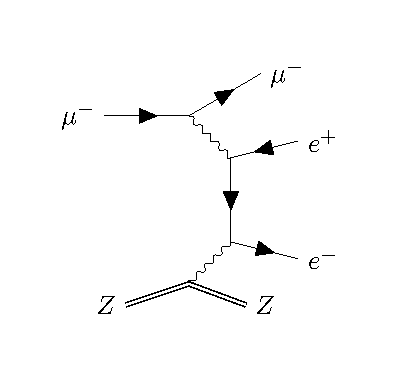
\includegraphics[trim=25 25 30 30, clip, width=0.6\textwidth]{images/feynman/epair_feynman.pdf}
        \end{minipage}%
        \end{column}
        \begin{column}{0.05\textwidth}
          \vspace{12mm}\\
          \Huge\textbf{\rightarrow}
        \end{column}
        \begin{column}{0.45\textwidth}
          \centering
            \textbf{Event signatures:}
            \begin{minipage}[c]{\textwidth}
              \vspace{4mm}
            \centering
                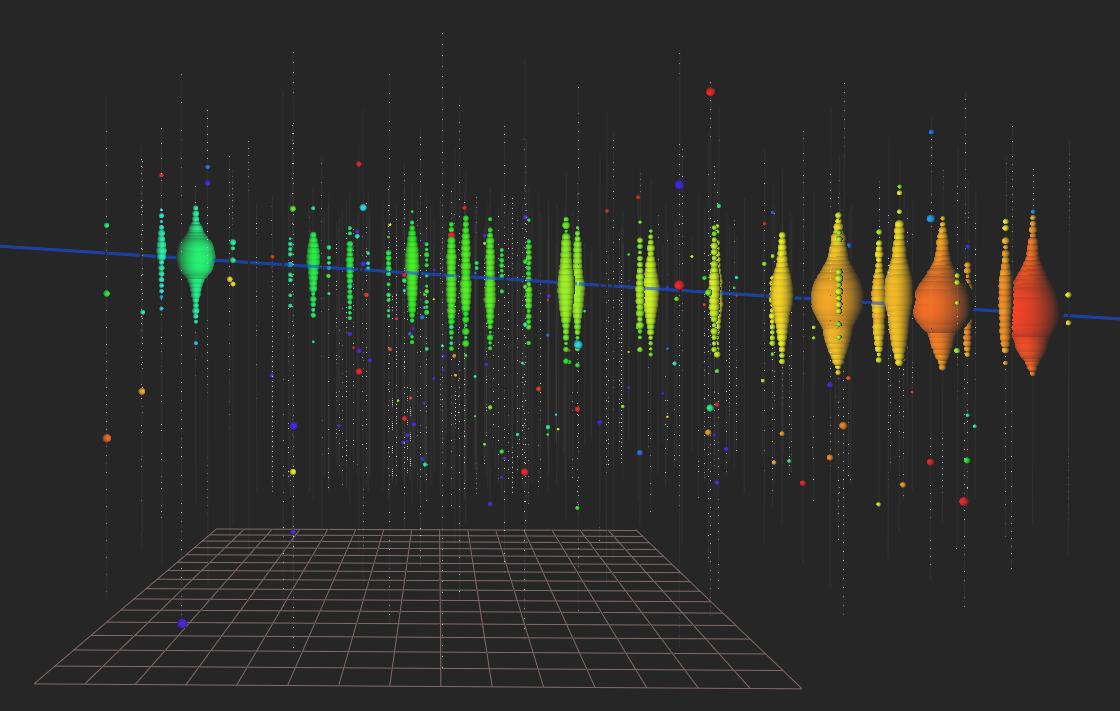
\includegraphics[width=0.8\textwidth]{images/Track.png}
                \credit{IceCube Collaboration}
        \end{minipage}%
        \end{column}
    \end{columns}
\end{frame}


\begin{frame}{}
  \vspace{-3cm}
  \begin{minipage}[t][1cm][t]{\textwidth}
  {\huge \textbf{PROPOSAL}} {\huge\textbf{\rightarrow}}
  \pgfsetfillopacity{0}\colorbox{tugreen}{\pgfsetfillopacity{1}{\huge \textbf{P}}{\Large ropagator}}{\Large with}\pgfsetfillopacity{0}\colorbox{tugreen}{\pgfsetfillopacity{1}{\huge \textbf{O}}{\Large ptimal }{\huge \textbf{P}}{\Large recision and }{\huge \textbf{O}}{\Large ptimized }{\huge \textbf{S}}{\Large peed}}{\Large for}\pgfsetfillopacity{0}\colorbox{tugreen}{\pgfsetfillopacity{1}{\huge \textbf{A}}ll {\huge \textbf{L}}{\Large eptons}}
  \end{minipage}
  \begin{minipage}[t][1cm][t]{\textwidth}
    
  \end{minipage}
\end{frame}

\begin{frame}{}
  \vspace{-3cm}
  \begin{minipage}[t][1cm][t]{\textwidth}
  {\huge \textbf{PROPOSAL}} {\huge\textbf{\rightarrow}}
  \pgfsetfillopacity{0.9}\colorbox{tugreen}{\pgfsetfillopacity{1}{\huge \textbf{P}}{\Large ropagator}}{\Large with}\pgfsetfillopacity{0}\colorbox{tugreen}{\pgfsetfillopacity{1}{\huge \textbf{O}}{\Large ptimal }{\huge \textbf{P}}{\Large recision and }{\huge \textbf{O}}{\Large ptimized }{\huge \textbf{S}}{\Large peed}}{\Large for}\pgfsetfillopacity{0}\colorbox{tugreen}{\pgfsetfillopacity{1}{\huge \textbf{A}}ll {\huge \textbf{L}}{\Large eptons}}
  \end{minipage}
  \begin{minipage}[t][1cm][t]{\textwidth}
  \vspace{-5mm}
    \begin{columns}[onlytextwidth]
        \begin{column}{0.5\textwidth}
            \begin{itemize}
              \item 3D Monte Carlo simulation of individual particles, considering \ldots
              \begin{itemize}
                \item[\normalcolor{\ldots}] energy losses
                \item[\normalcolor{\ldots}] scattering effects
                \item[\normalcolor{\ldots}] particle decays
              \end{itemize}
              \item \textbf{Input:} Initial particle state
              \item \textbf{Output:} Information on particle track, including \ldots
              \begin{itemize}
                \item[\normalcolor{\ldots}] Final particle state
                \item[\normalcolor{\ldots}] Energy losses
                \item[\normalcolor{\ldots}] Intermediate particle states
              \end{itemize}
            \end{itemize}
        \end{column}
        \begin{column}{0.5\textwidth}
            \begin{figure}
                \centering
                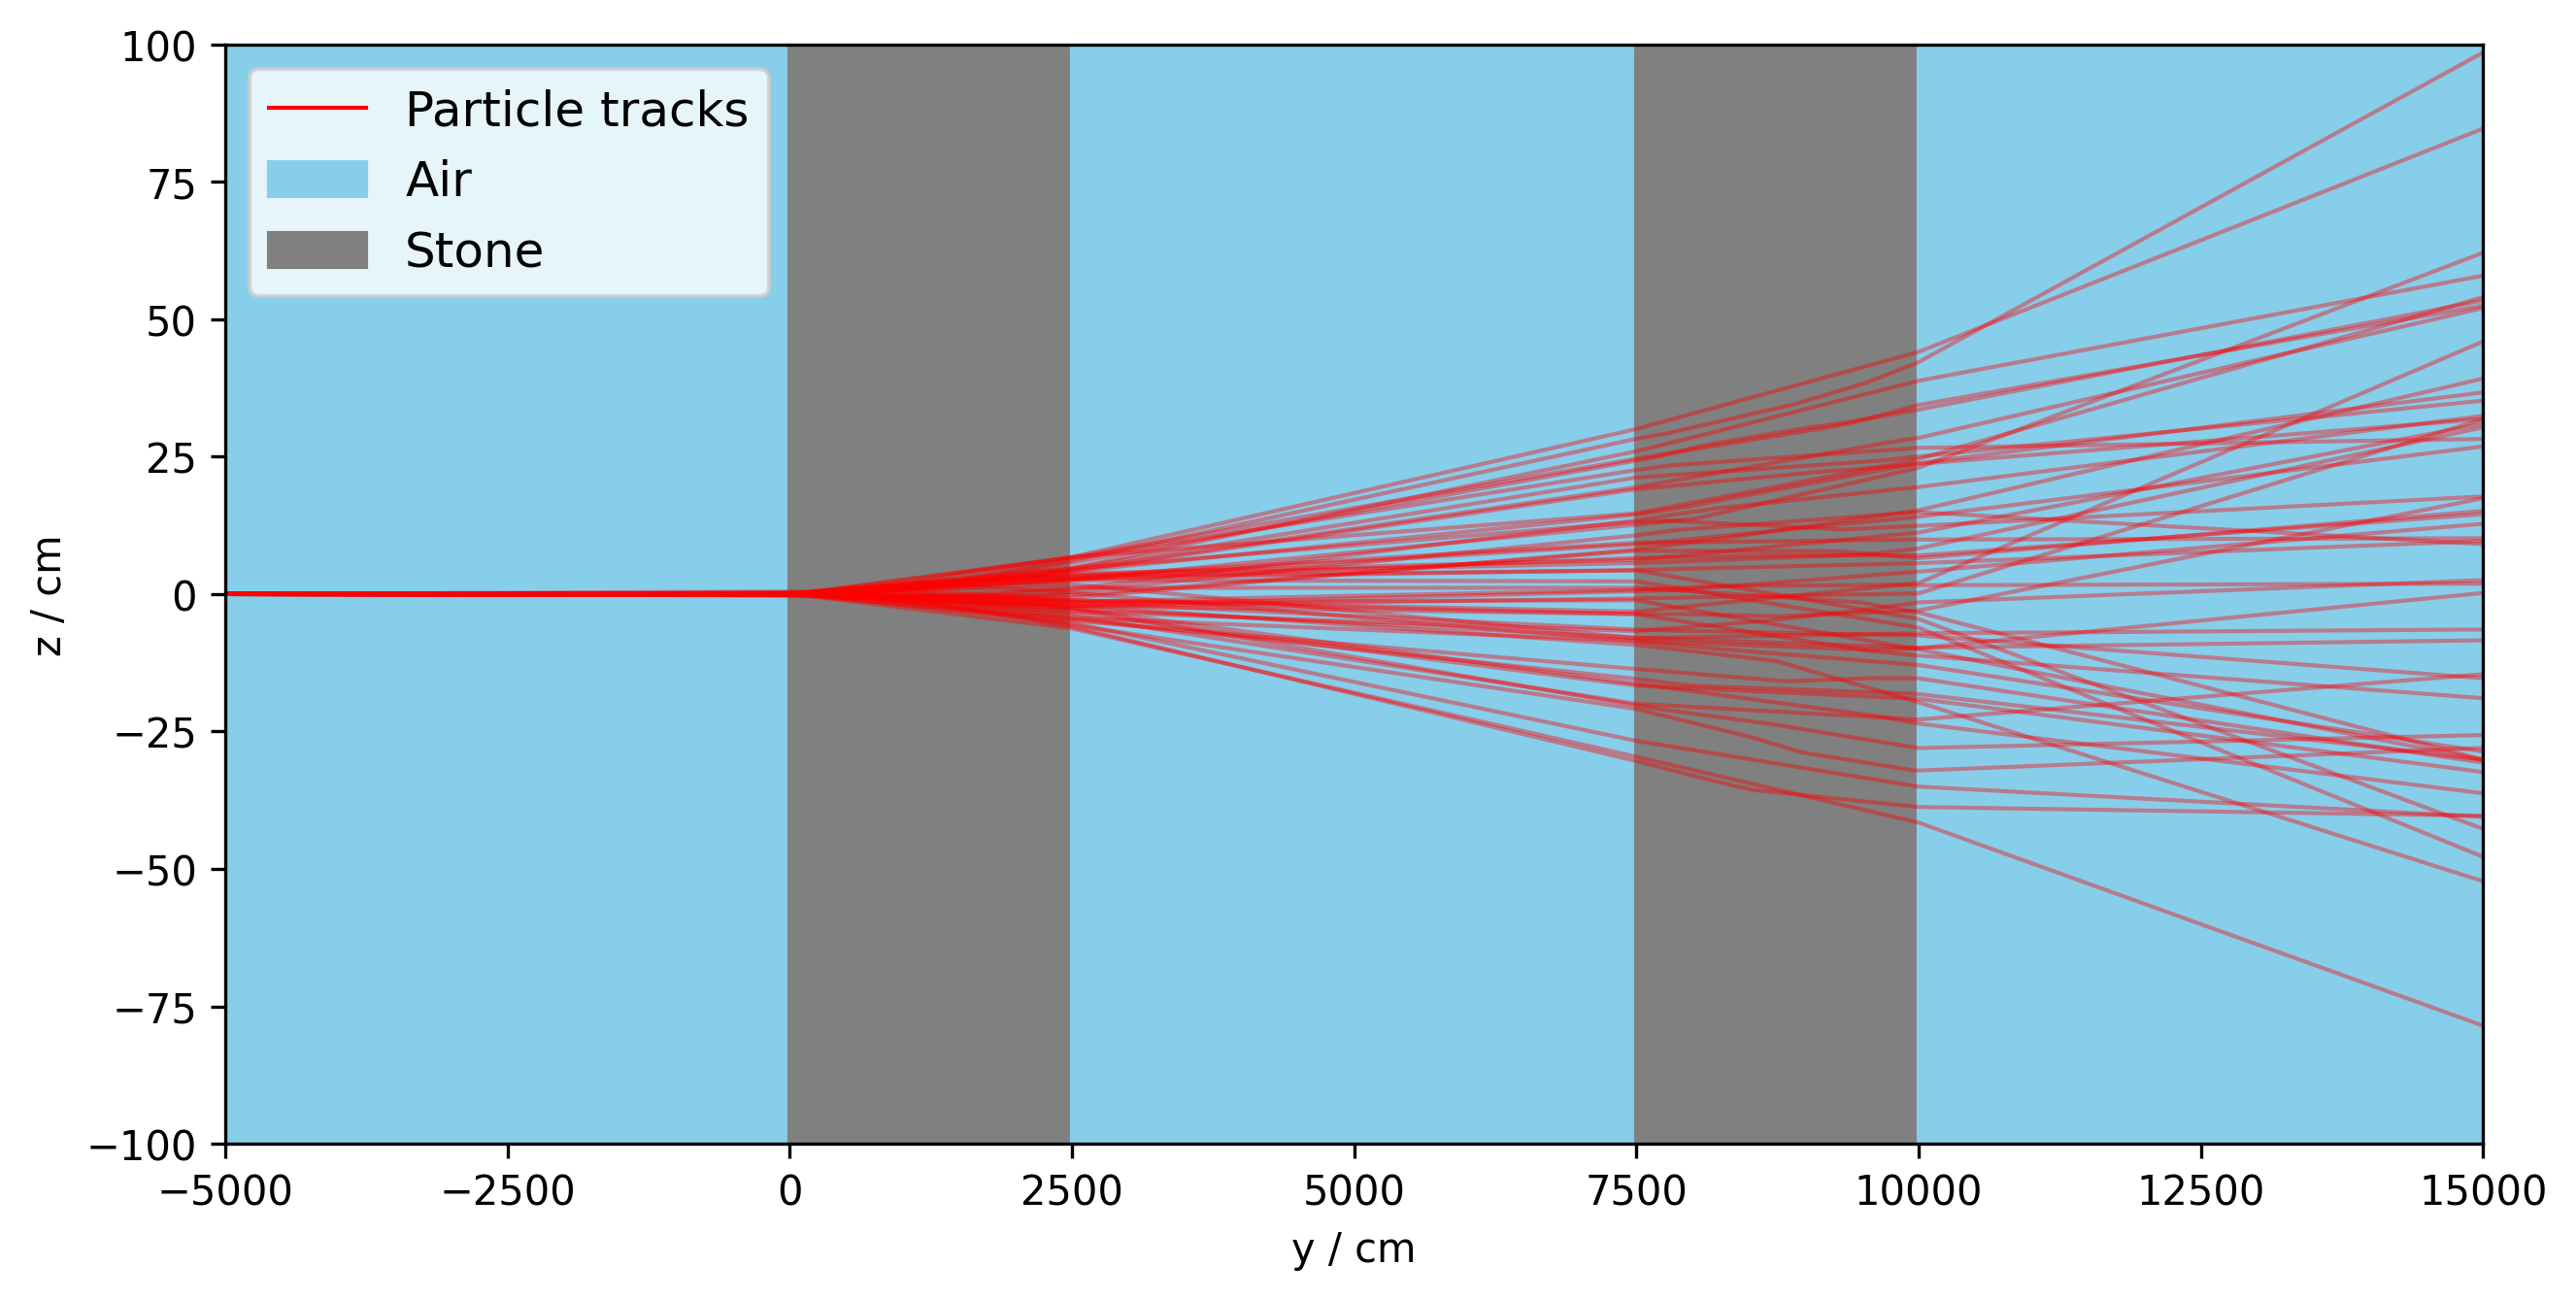
\includegraphics[width=0.85\textwidth]{plots/tracks.png}
            \end{figure}
            \vspace{-3mm}
            \begin{figure}
                \centering
                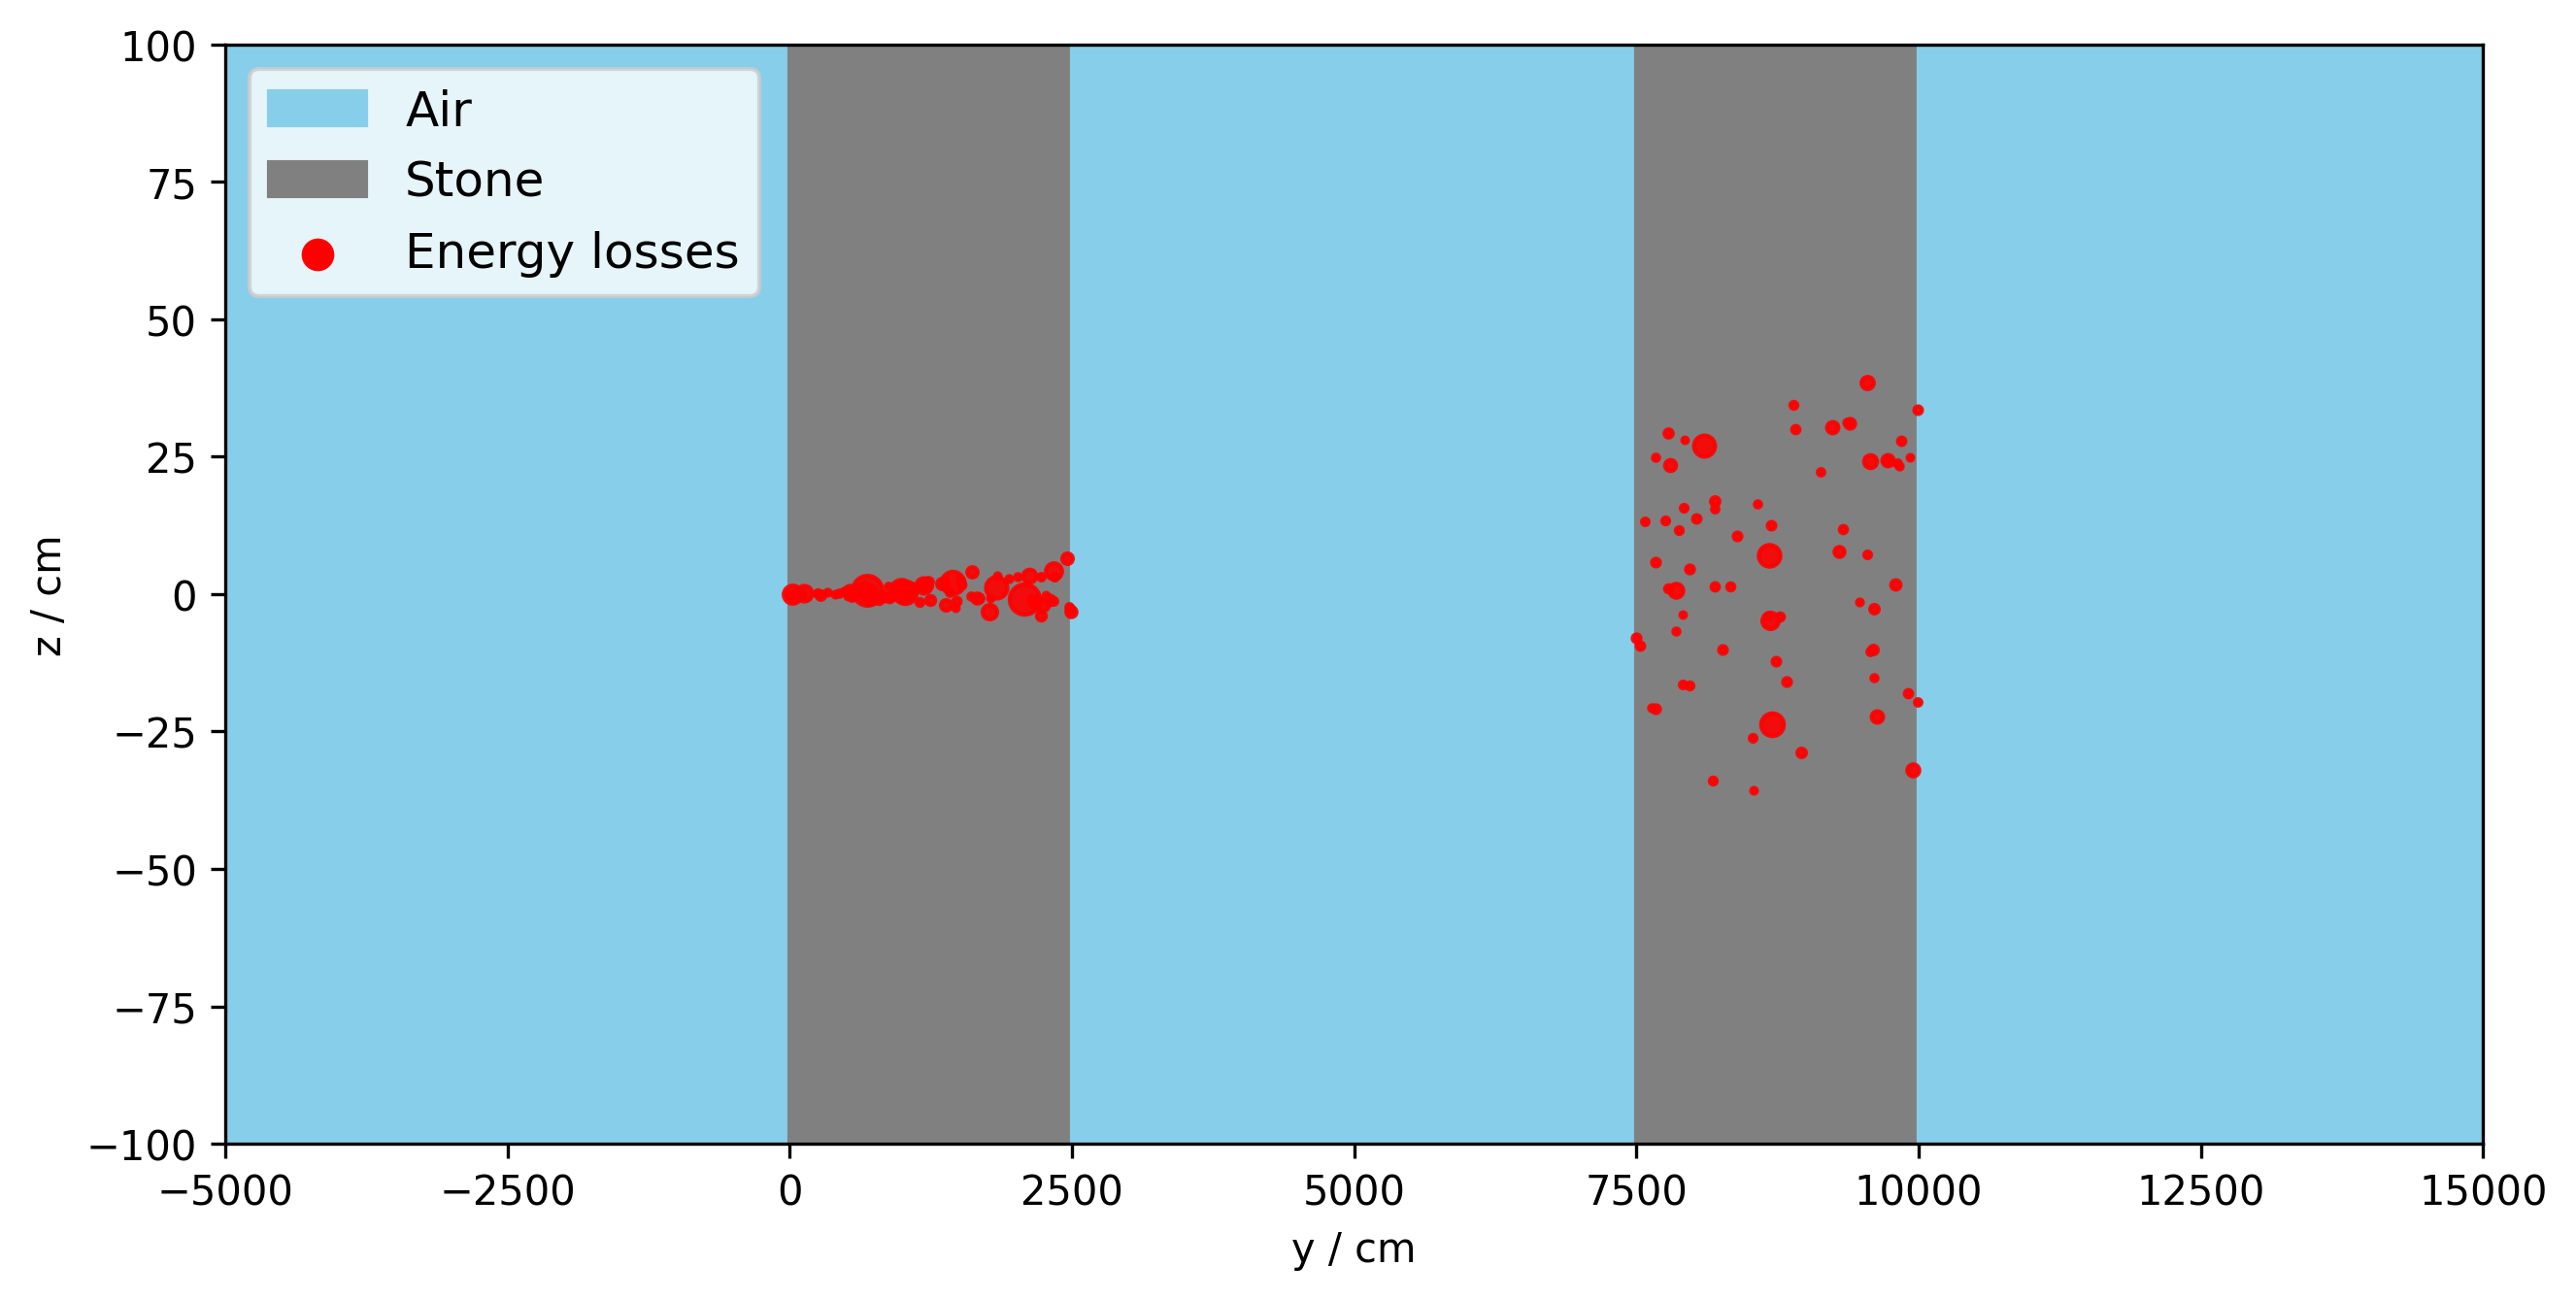
\includegraphics[width=0.85\textwidth]{plots/losses.png}
            \end{figure}
        \end{column}
    \end{columns}

  \end{minipage}
\end{frame}


\begin{frame}{}
  \vspace{-3cm}
  \begin{minipage}[t][1cm][t]{\textwidth}
  {\huge \textbf{PROPOSAL}} {\huge\textbf{\rightarrow}}
  \pgfsetfillopacity{0}\colorbox{tugreen}{\pgfsetfillopacity{1}{\huge \textbf{P}}{\Large ropagator}}{\Large with}\pgfsetfillopacity{0.9}\colorbox{tugreen}{\pgfsetfillopacity{1}{\huge \textbf{O}}{\Large ptimal }{\huge \textbf{P}}{\Large recision and }{\huge \textbf{O}}{\Large ptimized }{\huge \textbf{S}}{\Large peed}}{\Large for}\pgfsetfillopacity{0}\colorbox{tugreen}{\pgfsetfillopacity{1}{\huge \textbf{A}}ll {\huge \textbf{L}}{\Large eptons}}
  \end{minipage}
  \begin{minipage}[t][1cm][t]{\textwidth}
    \begin{columns}[onlytextwidth]
        \begin{column}{0.5\textwidth}
          \textbf{Interpolation tables:}
            \begin{itemize}
              \item Cross sections and results of propagation integrals are stored as interpolation tables
              \begin{itemize}
                %\item[$\rightarrow$] We use the \href{https://github.com/tudo-astroparticlephysics/cubic_interpolation}{CubicInterpolation} library 
                \item[$\rightarrow$] Crucial for the performance of PROPOSAL
              \end{itemize}
            \end{itemize}
          \textbf{Energy cuts:}
          \begin{itemize}
            \item Energy losses can be defined by their relative size $v_\text{loss}$ and their absolute size $e_\text{loss}$
            \item PROPOSAL differentiates between continuous and stochastic energy losses
            \item The energy cut settings ($v_\text{cut}, e_\text{cut}$) define which interaction are treated stochastically/continuously
            %\begin{itemize}
            %  \item[$\rightarrow$] Adjust energy cut settings to find ideal trade-off between precision and performance
            %\end{itemize}
          \end{itemize}
        \end{column}
        \begin{column}{0.5\textwidth}

          \begin{figure}
            \tikzstyle{vspecies_blue}=[rectangle, minimum size=0.5cm,draw=black,fill=blue, fill opacity=0.5, text opacity=1]
            \tikzstyle{vspecies_red}=[rectangle, minimum size=0.5cm,draw=black,fill=red, fill opacity=0.5, text opacity=1]

            \begin{tikzpicture}[>=latex,shorten >=2pt,shorten <=2pt,shape aspect=1]


            \coordinate (A) at (0, 0);

            \draw[draw=none, fill=blue, fill opacity=0.5] ($ (A) + (-3,-2) $) rectangle ++(6, 4);

            \draw[draw=none,fill=red, fill opacity=0.5] ($ (A) + (0, 0.07) $) circle (7.ex);

            \node [cylinder, shape border rotate=90, draw,minimum height=1cm,minimum width=0.75cm] (c) at (A) {};

            \node [vspecies_blue] (a) at (-1.1, 2.5) {\small{$v_\text{cut} = \num{0.05}$}} ;
            \node [vspecies_red] (b) at (1.1, 2.5) {\small{$e_\text{cut} = \SI{500}{\mega\electronvolt}$}} ;

            \draw [->] (-3, 0.7) -- (0, 0) node [midway, above, sloped] (TextNode) {$\mu$};

            \end{tikzpicture}
            \captionsetup{justification=centering}
            \caption*{$\rightarrow$ Adjust energy cut settings to find ideal \\trade-off between precision and performance!}
          \end{figure}

        \end{column}
    \end{columns}
  \end{minipage}
\end{frame}

\begin{frame}{}
  \vspace{-3cm}
  \begin{minipage}[t][1cm][t]{\textwidth}
  {\huge \textbf{PROPOSAL}} {\huge\textbf{\rightarrow}}
  \pgfsetfillopacity{0}\colorbox{tugreen}{\pgfsetfillopacity{1}{\huge \textbf{P}}{\Large ropagator}}{\Large with}\pgfsetfillopacity{0}\colorbox{tugreen}{\pgfsetfillopacity{1}{\huge \textbf{O}}{\Large ptimal }{\huge \textbf{P}}{\Large recision and }{\huge \textbf{O}}{\Large ptimized }{\huge \textbf{S}}{\Large peed}}{\Large for}\pgfsetfillopacity{0.9}\colorbox{tugreen}{\pgfsetfillopacity{1}{\huge \textbf{A}}ll {\huge \textbf{L}}{\Large eptons}}
  \end{minipage}
  \begin{minipage}[t][1cm][t]{\textwidth}
    
  \vspace{-20pt}
  \begin{columns}[t]
    \column{.5\textwidth}
    \begin{figure}
      \caption*{Muon energy losses:}
      \vspace{-9pt}
      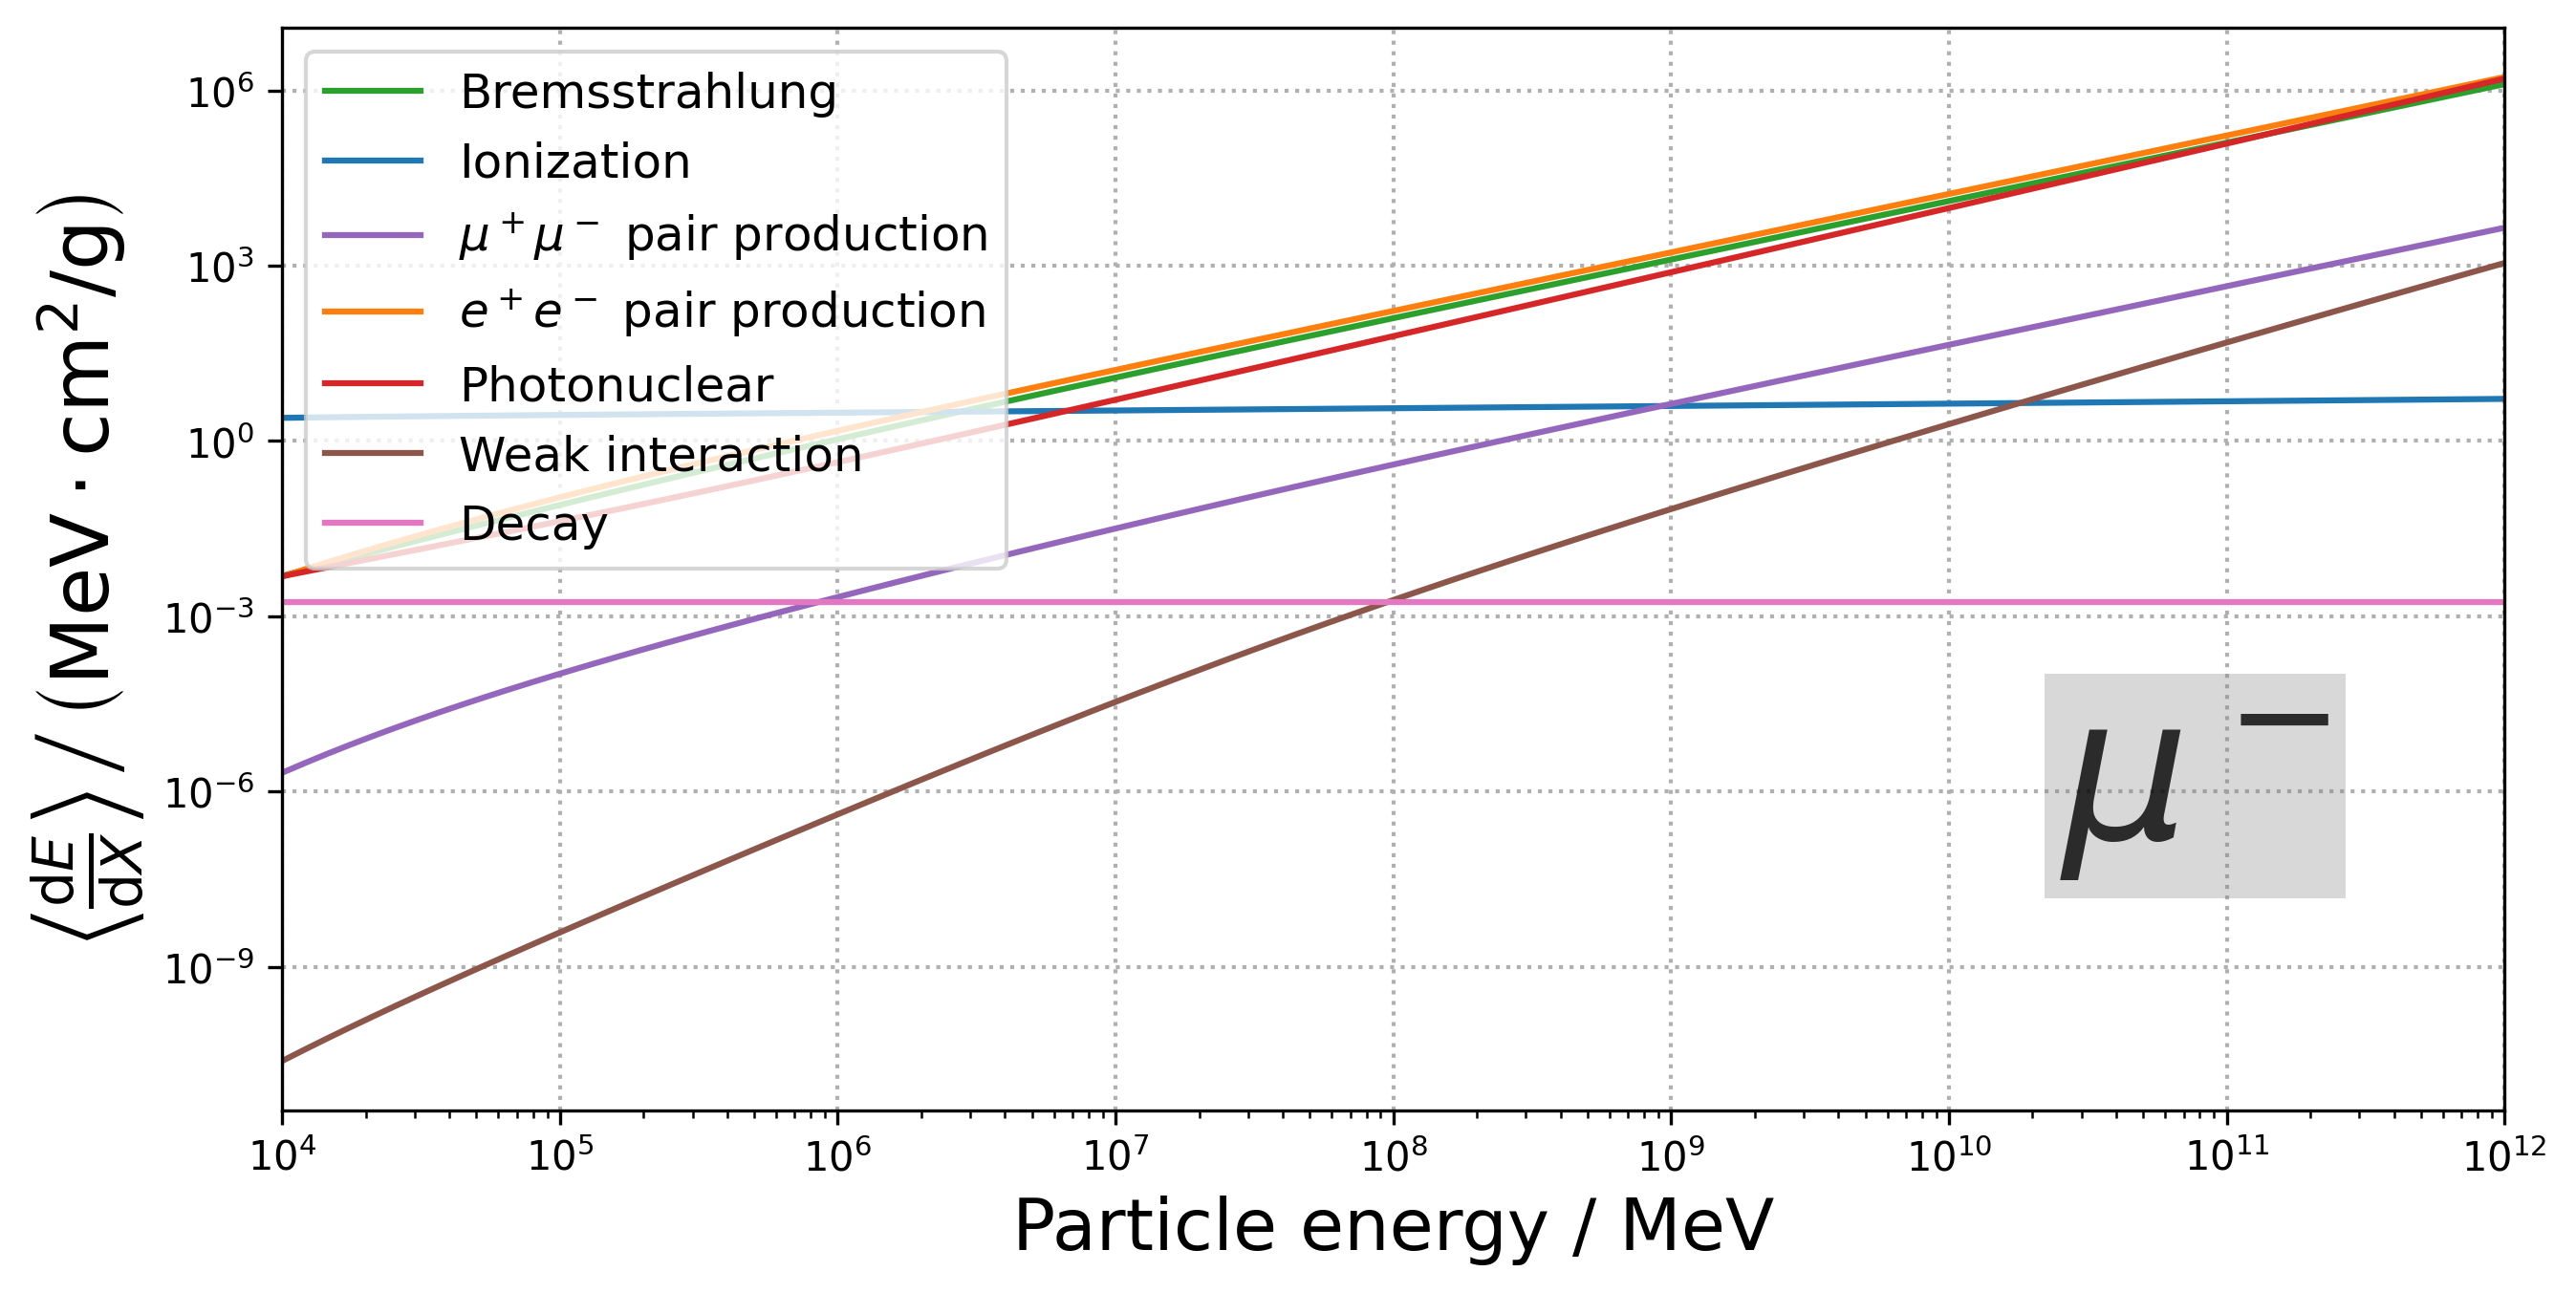
\includegraphics[width=\linewidth, height=.37\textheight, keepaspectratio]{plots/muon_dEdx.png}
    \end{figure}
    \vspace{-15pt}
    \begin{figure}
      \caption*{Positron/Electron energy losses:}
      \vspace{-9pt}
      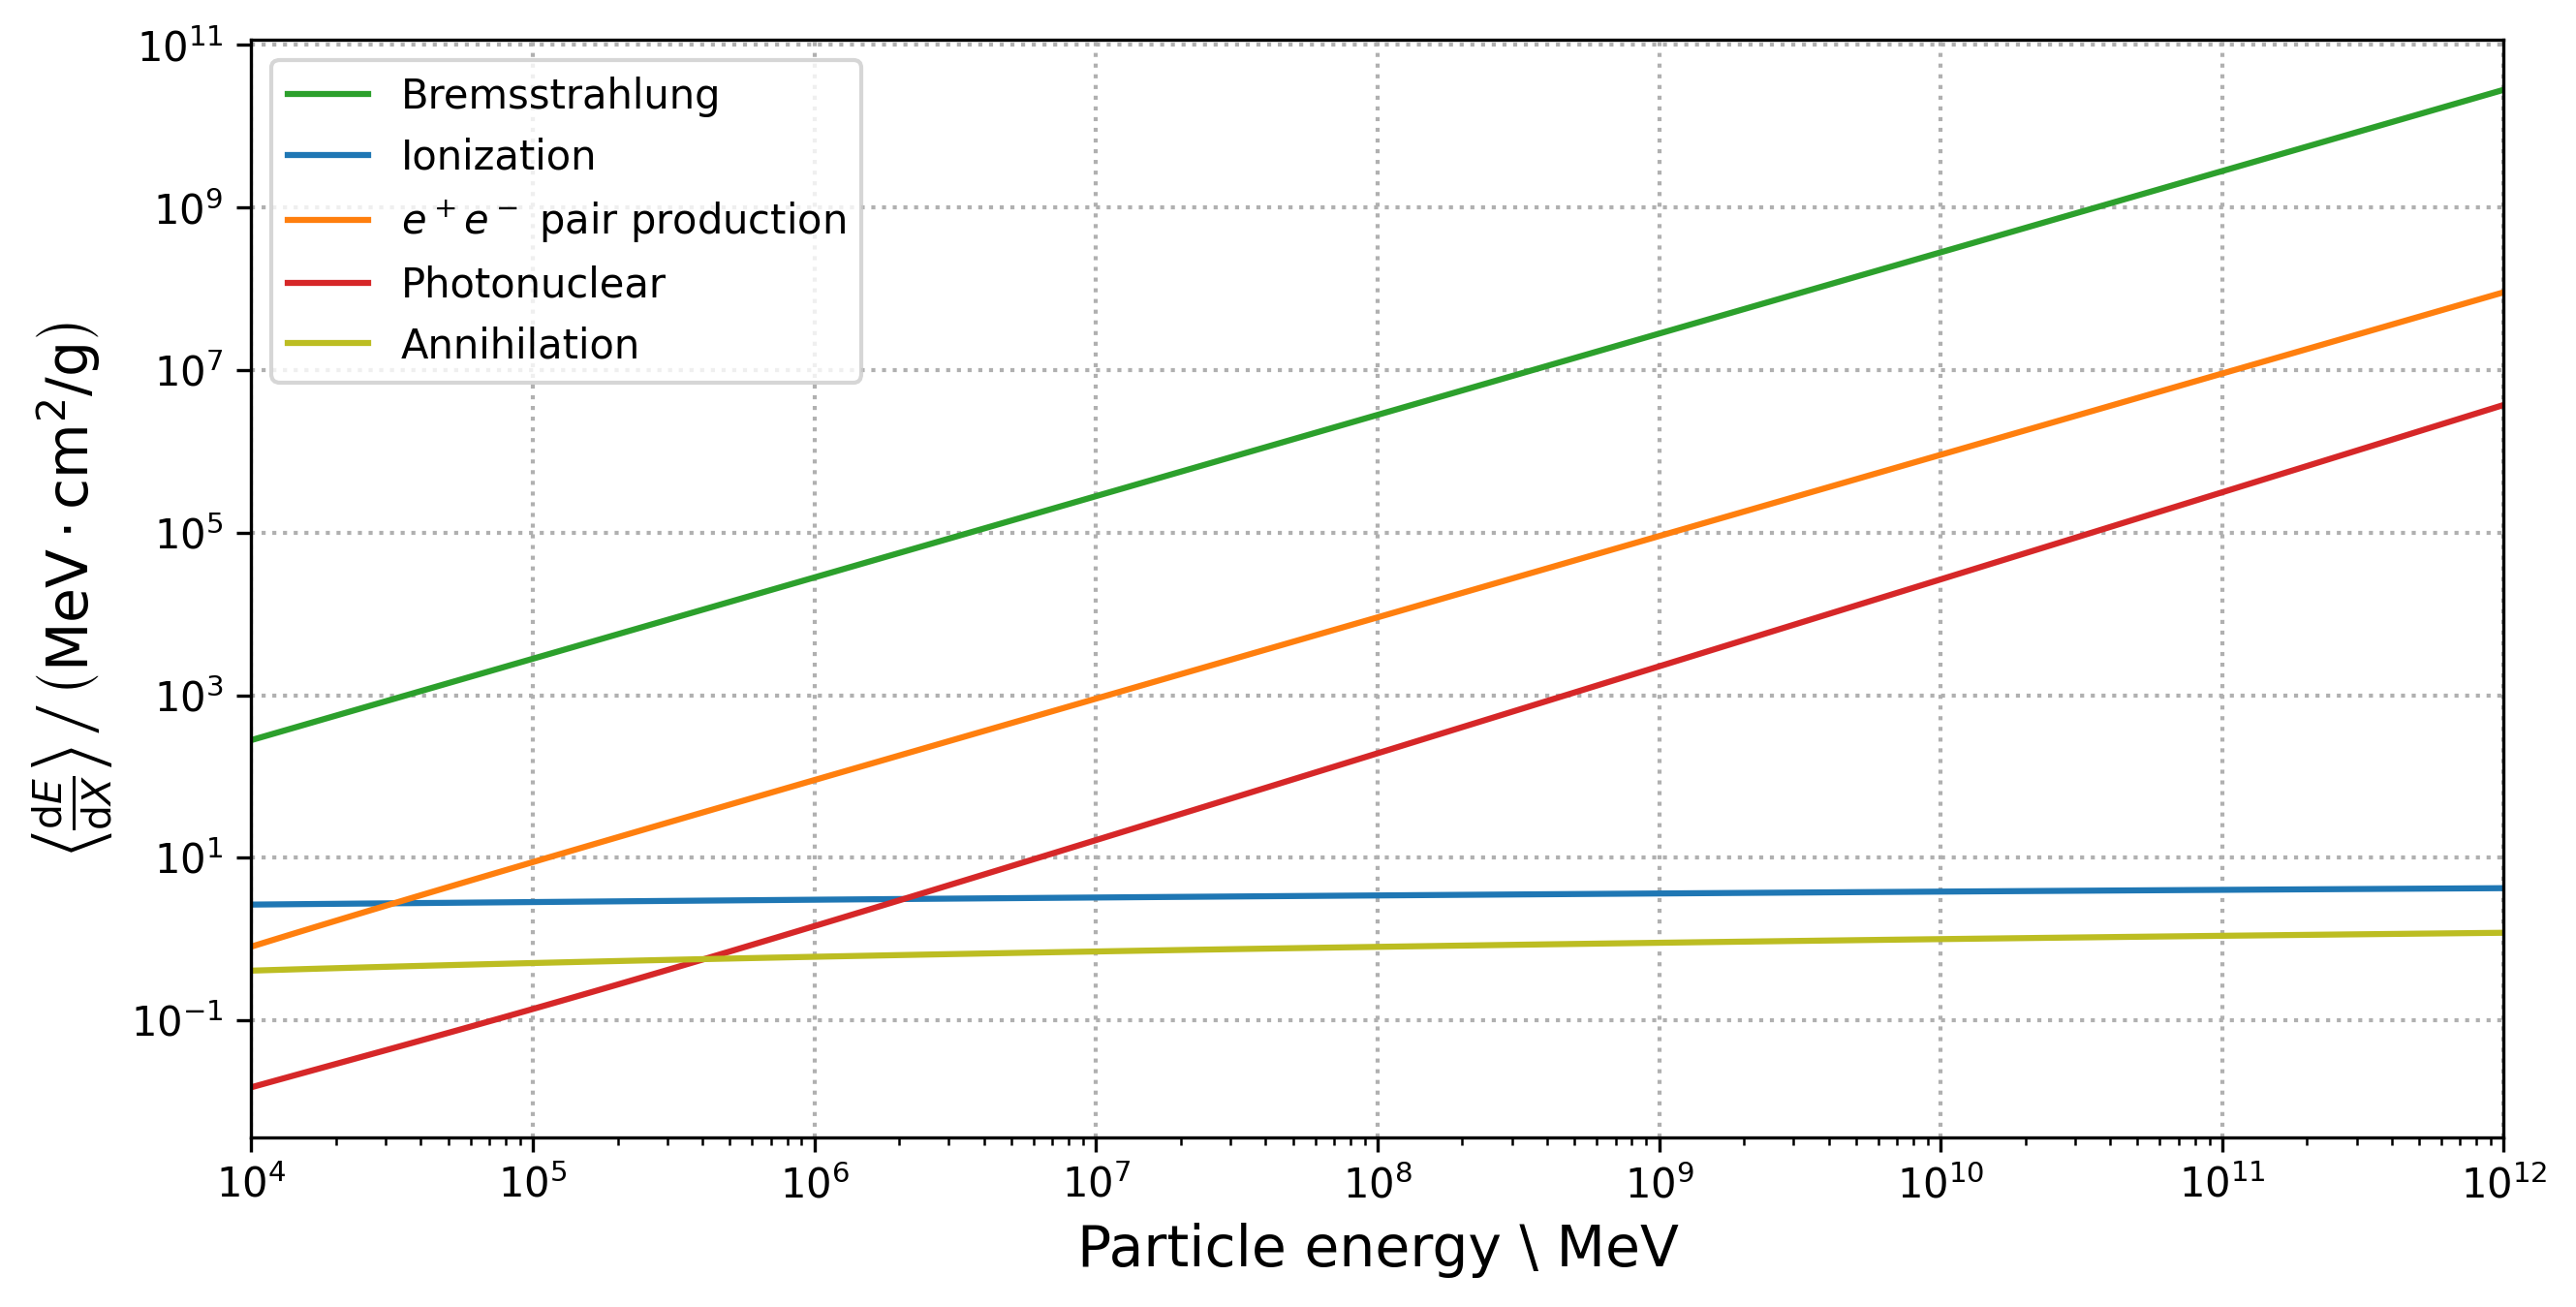
\includegraphics[width=\linewidth, height=.37\textheight, keepaspectratio]{plots/positron_dEdx.png}
    \end{figure}
    \vspace{-20pt}
    \column{.5\textwidth}
    \begin{figure}
      \caption*{Tau energy losses:}
      \vspace{-9pt}
      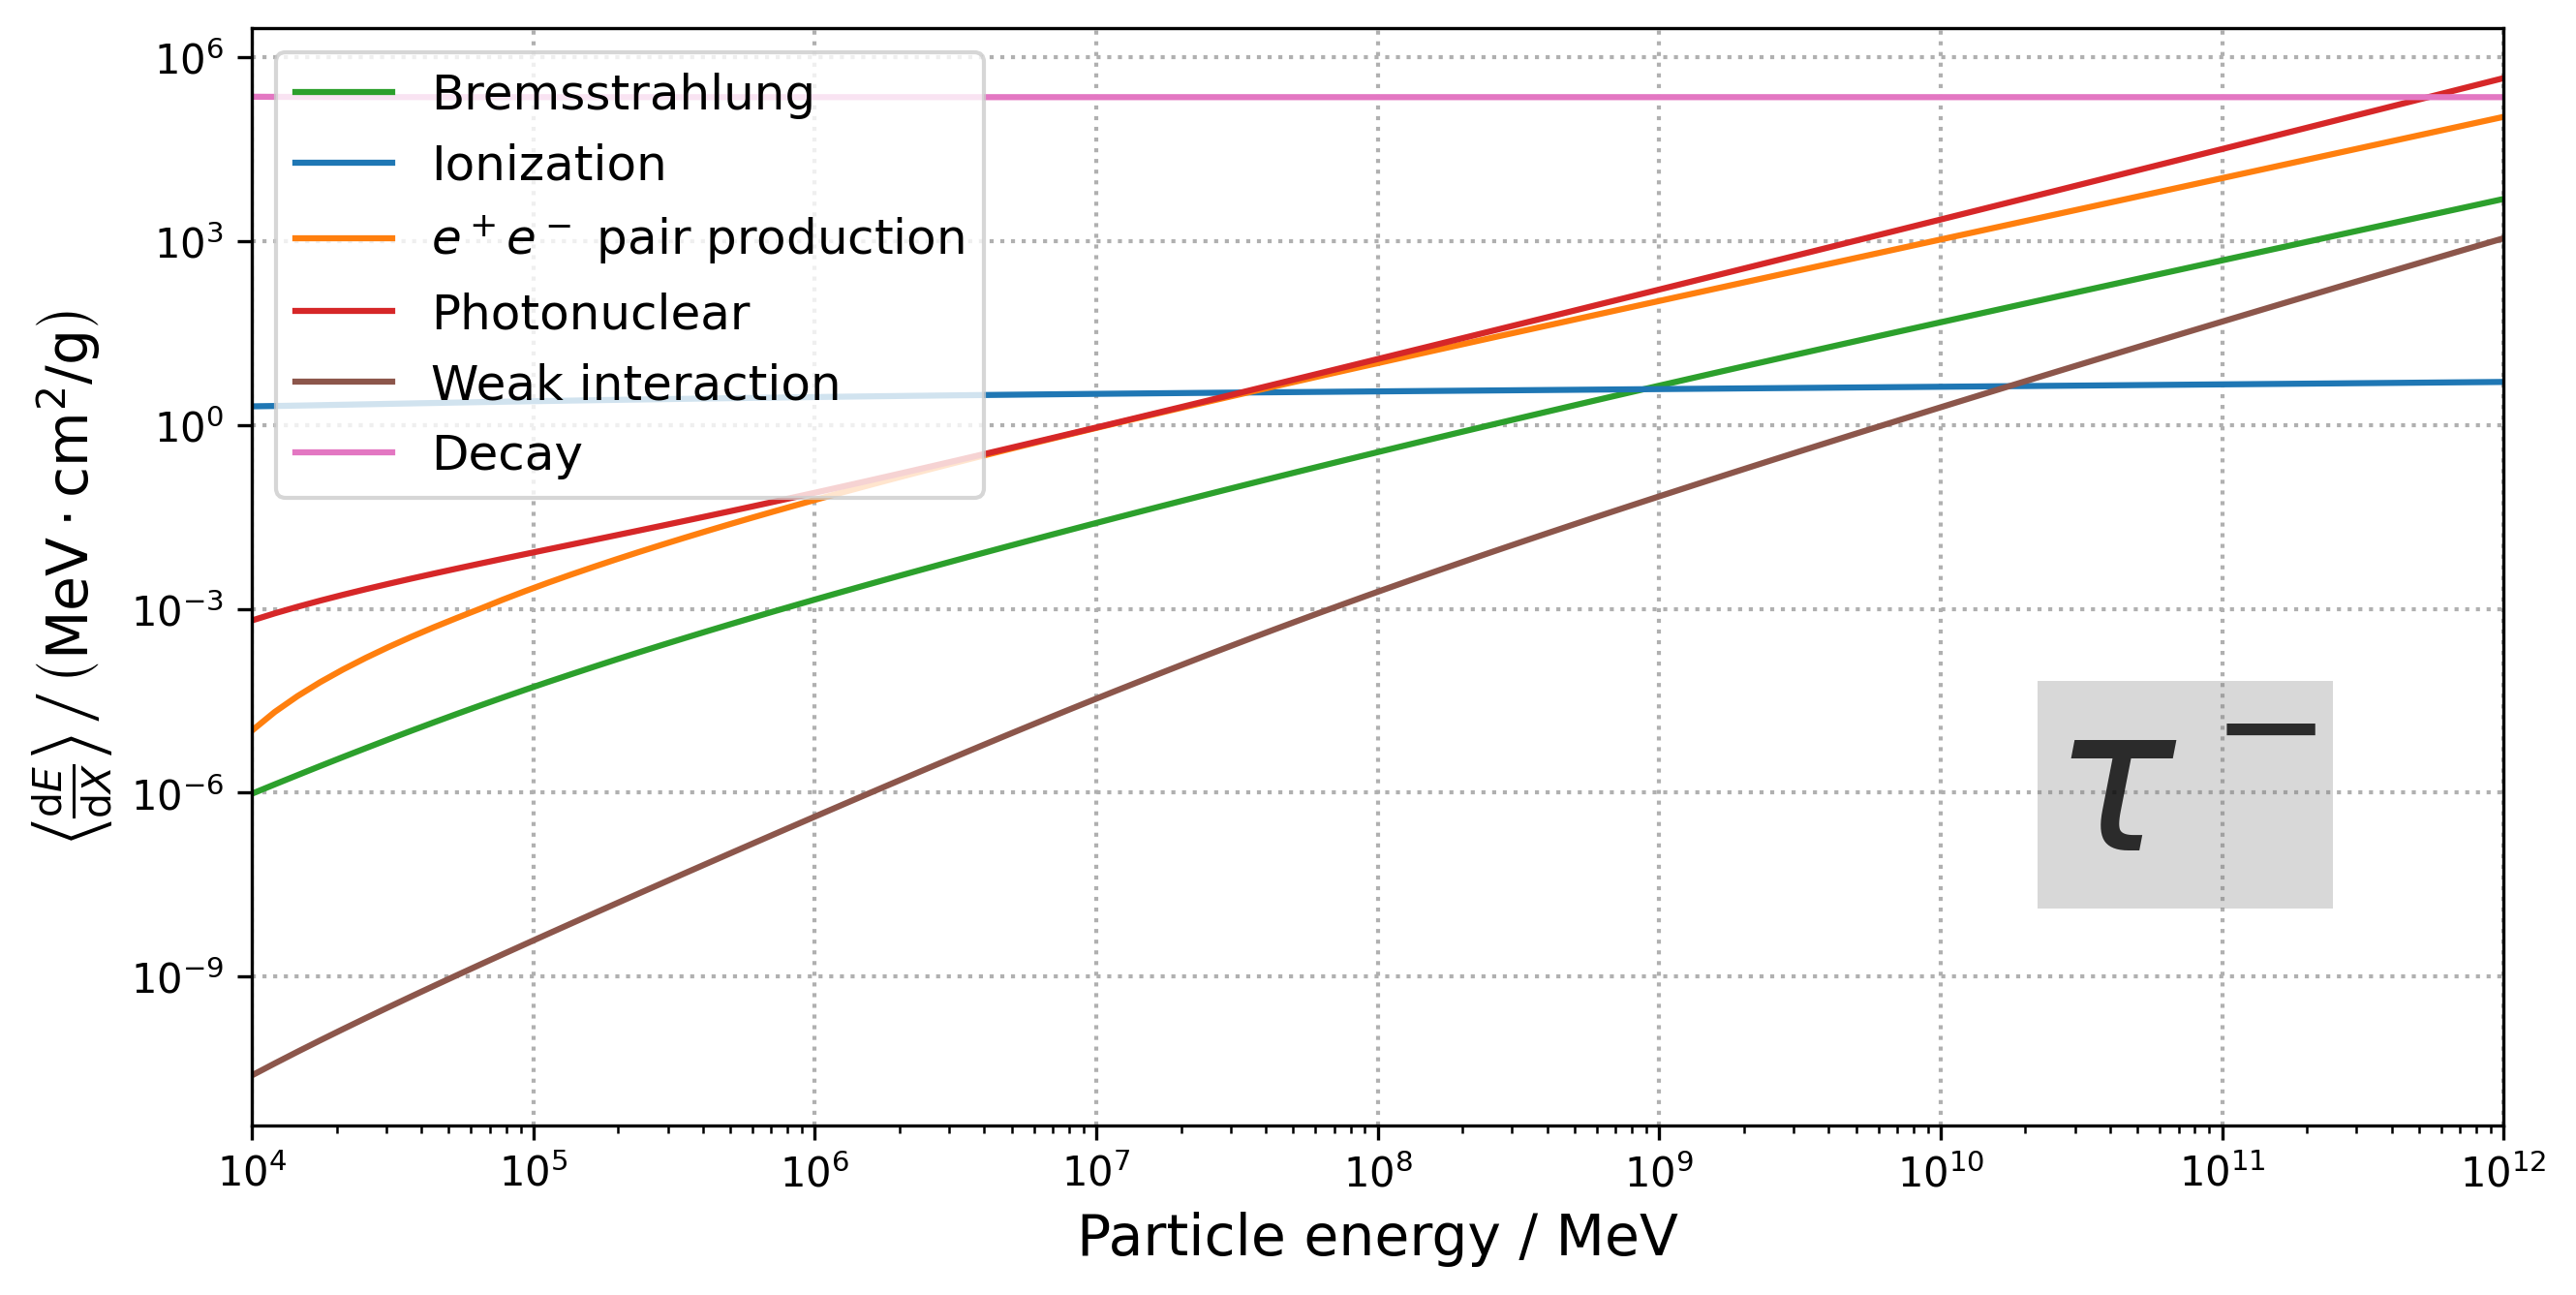
\includegraphics[width=\linewidth, height=.37\textheight, keepaspectratio]{plots/tau_dEdx.png}
    \end{figure}
    \vspace{-15pt}
    \begin{figure}
      \caption*{High-energy photon energy losses:}
      \vspace{-9pt}
      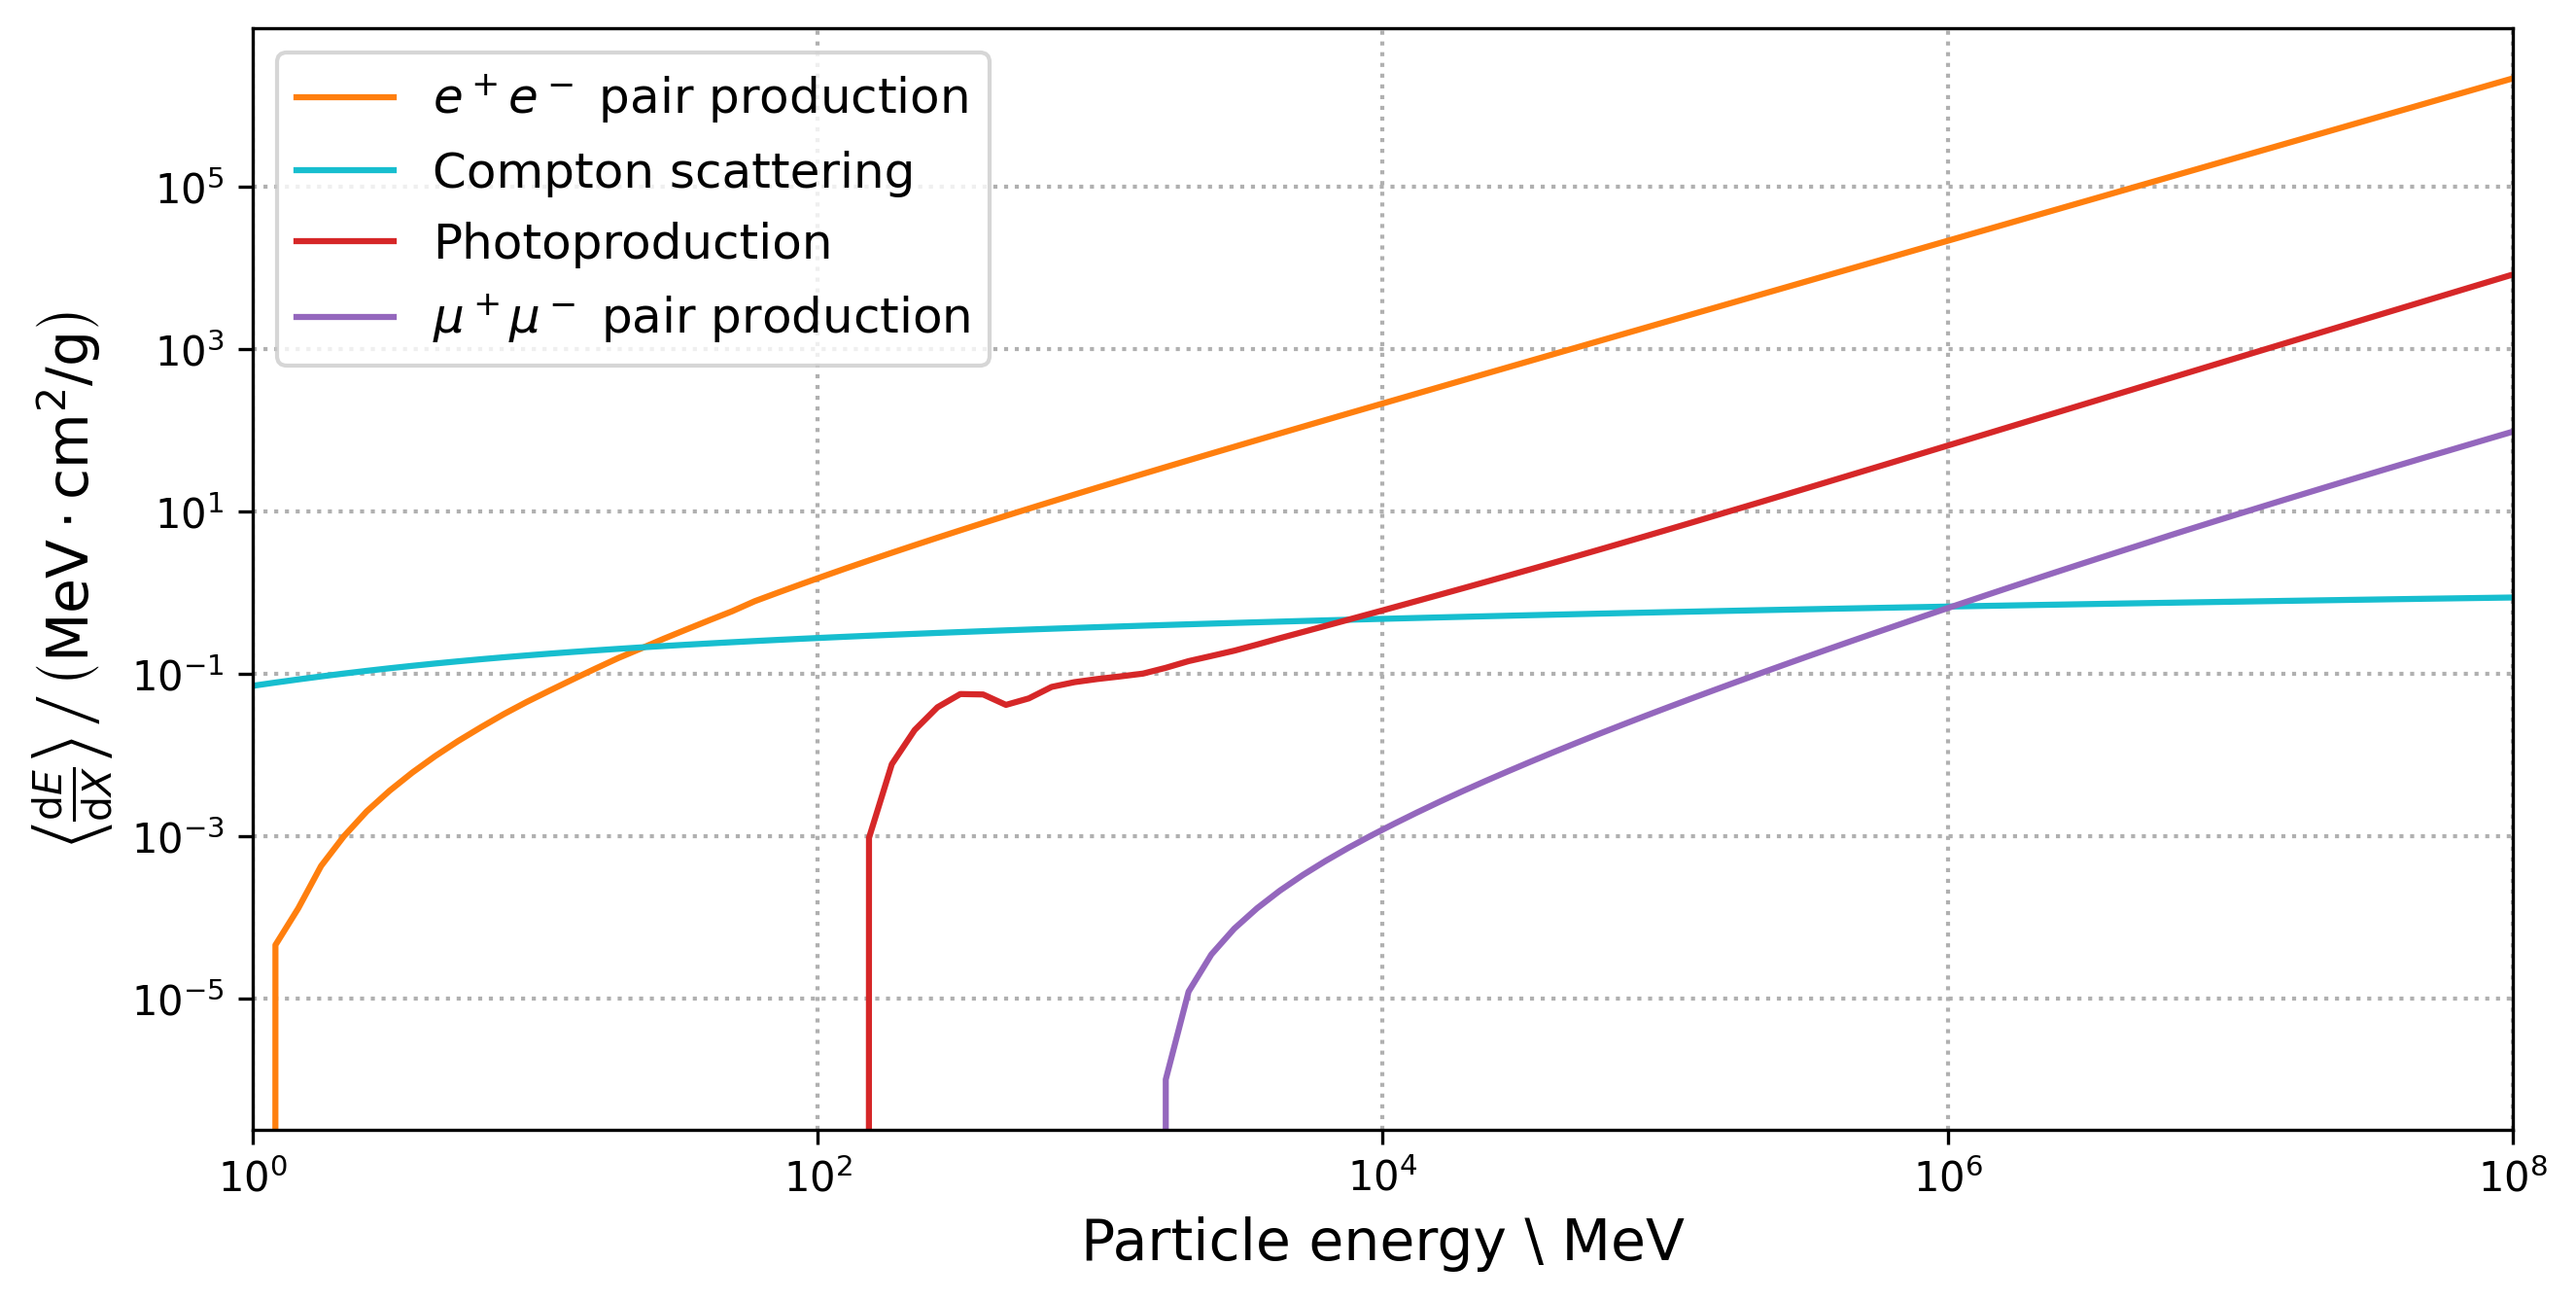
\includegraphics[width=\linewidth, height=.37\textheight, keepaspectratio]{plots/photon_dEdx.png}
    \end{figure}
  \end{columns}

  \end{minipage}
\end{frame}